\documentclass{article}[12pt]
%\usepackage{fullpage}
%\usepackage{fullpage}
\usepackage{amsmath}
\usepackage{latexsym}
\usepackage{amssymb,amsfonts}
\usepackage{graphicx}
\usepackage{graphics}
\usepackage[margin=.75in]{geometry}

\graphicspath{ {../../assets/} }

\begin{document}

\large


\newcommand{\activityname}{
  Secret of Nim
}
\newcommand{\subtitle}{
  It's all fun and Game Theory
}

\phantom{.}\hspace{-.5in}\begin{tabular}{lr}
 \begin{tabular}{l}
    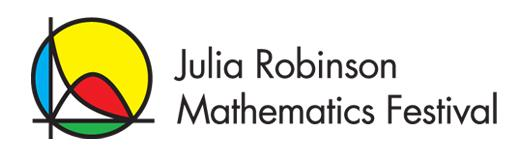
\includegraphics[width=3in]{jrmcf-logo.jpg}
 \end{tabular}
 & \hspace{1in}
 \begin{tabular}{r}
    {\Huge \activityname}\\
    {\subtitle}
 \end{tabular}
\end{tabular}
\thispagestyle{empty}

\noindent\hrulefill
\phantom{.}\vspace{.15in}

\textbf{Game theory} is the mathematical study of decisions and games.
Play the below games and try to answer the following questions.

\bigskip\bigskip

\noindent\textbf{\huge Take Away}

\begin{itemize}
\item \textbf{Setup:} Roll three six-sided dice. Add up their values, then place
that many coins on the table.
\item \textbf{Gameplay:} Players alternate taking one, two, or three coins
from the table.
\item \textbf{Object:} The winner is the player who takes the last coin from
the table.
\end{itemize}

\noindent{\Large Questions}

\begin{itemize}
\item Which kinds of dice rolls are better for the first player?
\item Which kinds of dice rolls are better for the second player?
\item Which player wins most often in this game?
\end{itemize}

\bigskip\bigskip

\noindent\textbf{\huge Nim}

\begin{itemize}
\item \textbf{Setup:} Roll three six-sided dice. For each die, place that
many pennies, nickels, and dimes on the table.
\item \textbf{Gameplay:} Players alternate one or more coins of the same
type from the table.
\item \textbf{Object:} The winner is the player who takes the last coin from
the table.
\end{itemize}

\noindent{\Large Questions}

\begin{itemize}
\item Which kinds of dice rolls are better for the first player?
\item Which kinds of dice rolls are better for the second player?
\end{itemize}

\input{../../footer.tex}